% \documentclass[manuscript, screen=true, review=true, anonymous=true, authordraft=False]{acmart}
\documentclass[sigconf]{acmart}

%%% START ADDITIONAL PACKAGES AND COMMANDS %%% 
\renewcommand{\sectionautorefname}{Section}
\renewcommand{\subsectionautorefname}{Section}
\renewcommand{\subsubsectionautorefname}{Section}

\usepackage{tabularx}
\usepackage{dcolumn} %Aligning numbers by decimal points in table columns
\newcolumntype{d}[1]{D{.}{.}{#1}}

\usepackage{subcaption}

\usepackage{todonotes}
\let\xtodo\todo
\renewcommand{\todo}[1]{\xtodo[inline,color=green!50]{#1}}
\newcommand{\itodo}[1]{\xtodo[inline]{#1}}
\newcommand{\red}[1]{\textcolor{red}{#1}}
\newcommand{\sven}[1]{\xtodo[inline,color=yellow!50]{Sven: #1}}
%%% END ADDITIONAL PACKAGES AND COMMANDS %%% 

%%
%% \BibTeX command to typeset BibTeX logo in the docs
\AtBeginDocument{%
  \providecommand\BibTeX{{%
    Bib\TeX}}}

%% Rights management information.  This information is sent to you
%% when you complete the rights form.  These commands have SAMPLE
%% values in them; it is your responsibility as an author to replace
%% the commands and values with those provided to you when you
%% complete the rights form.
\setcopyright{acmcopyright}
\copyrightyear{2018}
\acmYear{2018}
\acmDOI{XXXXXXX.XXXXXXX}

%% These commands are for a PROCEEDINGS abstract or paper.
\acmConference[Conference acronym 'XX]{Make sure to enter the correct
  conference title from your rights confirmation emai}{June 03--05,
  2018}{Woodstock, NY}
\acmPrice{15.00}
\acmISBN{978-1-4503-XXXX-X/18/06}


%%
%% Submission ID.
%% Use this when submitting an article to a sponsored event. You'll
%% receive a unique submission ID from the organizers
%% of the event, and this ID should be used as the parameter to this command.
%%\acmSubmissionID{123-A56-BU3}

%% A "teaser" image appears between the author and affiliation
%% information and the body of the document, and typically spans the
%% page.
%\begin{teaserfigure}
%  \includegraphics[width=\linewidth]{sampleteaser}
%  \caption{Seattle Mariners at Spring Training, 2010.}
%  \Description{Enjoying the baseball game from the third-base
%  seats. Ichiro Suzuki preparing to bat.}
%  \label{fig:teaser}
%\end{teaserfigure}


%%
%% end of the preamble, start of the body of the document source.
\begin{document}

%%
%% The "title" command has an optional parameter,
%% allowing the author to define a "short title" to be used in page headers.
\title{% Preserving Agency in Human Augmentation using Brain Signals reflecting the Intent to Interact

% Preserving Agency in Action Augmentation using Brain Signals reflecting the Intent to Interact

% Intended Augmentation: Preserving Agency for Augmented Humans using Brain Signals reflecting the Intent to Interact

% Preserving Agency for Augmented Humans using Brain Signals reflecting the Intent to Interact

% Preserving Agency During Action Augmentation using Brain Signals of the Intent to Interact

% AAA: Agency-preserving Action Augmentation using Brain-Computer Interfaces
% Brain Signals of the Intent to Interact

% Agency-preserving Human Augmentation using Brain-Computer Interfaces

% - Agency-preserving Action Augmentation using Brain-Computer Interfaces

%Agency-preserving Action Augmentation using Brain Signals of the Intent to Interact

% - Supporting Agency Experience Using Brain-Computer Interface based Muscle Control 

Agency-preserving Action Augmentation: Towards Preemptive Muscle Control using Brain-Computer Interfaces

% - Supporting Augmented Agency Experiences Using Brain-Computer Interface based Muscle Control
% agencEEG

% staying in the driving seat of augmented actions}

%%
%% The "author" command and its associated commands are used to define
%% the authors and their affiliations.
%% Of note is the shared affiliation of the first two authors, and the
%% "authornote" and "authornotemark" commands
%% used to denote shared contribution to the research.

\settopmatter{authorsperrow=3}

\author{Lukas Gehrke}
\orcid{0000-0003-3661-1973}
\affiliation{%
  \institution{TU Berlin}
  \city{Berlin}
  \postcode{10623}
  \country{Germany}
}
\email{lukas.gehrke@tu-berlin.de}

\author{Leonie Terfurth}
\orcid{}
\affiliation{%
  \institution{TU Berlin}
  \city{Berlin}
  \postcode{10623}
  \country{Germany}
}
\email{leonie.terfurth@tu-berlin.de}

\author{Klaus Gramann}
\orcid{0000-0003-2673-1832}
\affiliation{%
  \institution{TU Berlin}
  \city{Berlin}
  \postcode{10623}
  \country{Germany}
}
\email{klaus.gramann@tu-berlin.de}

%%
%% By default, the full list of authors will be used in the page
%% headers. Often, this list is too long, and will overlap
%% other information printed in the page headers. This command allows
%% the author to define a more concise list
%% of authors' names for this purpose.
\renewcommand{\shortauthors}{Gehrke et al.}

%%
%% The abstract is a short summary of the work to be presented in the
%% article.
\begin{abstract}

% Besides the title, this is what most people (90+%) will read from your paper!

% - [ ] Therefore, improve SEO (Search engine optimization): copy the abstract text to hemingwayapp.com to improve information density, keyword frequency and readability! Go through each sentence to shorten it and remove unnecessary words.

abstract text there only

\listoftodos
\end{abstract}

%%
%% The code below is generated by the tool at http://dl.acm.org/ccs.cfm.
%% Please copy and paste the code instead of the example below.
%%

\begin{CCSXML}
<ccs2012>
    <concept_id>10003120.10003121.10003128</concept_id>
        <concept_desc>Human-centered computing~Human computer interaction (HCI)</concept_desc>
        <concept_significance>300</concept_significance>
    </concept>
 </ccs2012>
\end{CCSXML}
\ccsdesc[500]{Human-centered computing~Human computer interaction (HCI)}


%%
%% Keywords. The author(s) should pick words that accurately describe
%% the work being presented. Separate the keywords with commas.
\keywords{action augmentation, sense of agency, brain-computer interface, human computer interaction, intention}

%%
%% This command processes the author and affiliation and title
%% information and builds the first part of the formatted document.
\maketitle

\section{Introduction}
% 1. Describe the Current Situtation
% Functions as a starting point and a common basis. Therefore it primarily contains recognizable and agreed points.
% 2. What is the complication, challenge identified
% Spells the reason for acting now. It contains threats / opportunities and the hurdles that need to be overcome.
Technological advances in hardware that augment a user's physical actions have reignited dreams of overcoming human limitations, recovering lost abilities as well as simplifying skill acquisition. Wearable exoskeletons move a user's body by applying forces to the extremities, for example by pulling on the fingertips (see Dexmo Haptic Glove \footnote{https://www.dextarobotics.com/}) while electrical muscle stimulation (EMS) makes the user's extremities move by sending current into the muscle activating nerves. These technologies are becoming increasingly seamless to use. However, augmented user's frequently report dissociative experiences during or following augmented action. They do not experience agency.

The sense of agency refers to the experience of being in control of our own voluntary actions, instead of them feeling as though they randomly happen to us. This being in the "driving seat when it comes to our own actions"~\cite{Moore2016-ub} can be subdivided into the \textit{feeling} of agency, a low level pre-reflective sensory process, and a more higher level reflective cognitive process, the \textit{judgement} of agency~\cite{Moore2016-ub, Danry2022-xk}. The key challenge in human \textit{physical augmentation} is to create an experience of pre-reflective agency, so user's feel as though they are in the "driving seat" once again.
% if something happens for you in an interaction there is a cost to that:
% - impacts sense of agency which in turn makes user's engage less
% - impacts precision and accuracy, which can be very critical in high stakes scenarios, e.g. air traffic control

% 3. Question
% Asks the question how the hurdles of the Complication can be overcome. How can we prevent the threat or seize the opportunity? Also, what would be the benefits if the complication would be overcome?
% What have others done to address this and what do we propose "instead"
In physical augmentation, this experience of agency positively impacts performance.~\citet{Kasahara2019-sk} have shown that reaction times when tapping targets on a touchscreen can be increased by augmenting the user. Critically they found an optimal increase in reaction time, \textit{pre-emptive} gain, that preserves agency. At around 80 ms preceding the naturally occurring action, user's integrate the augmentation and maintain an experience of agency. However, setting this gain factor is dependent on each specific task and requires fitting the parameters over and over again. A key question remains: How can we maintain agency during physical augmentation without training and over-fitting parameters? In other words, how can we create closed systems for users to experience \textit{natural} augmentation?

% 4. (short) Answer Teaser
% Provides the answer on how to overcome the hurdles. Explains how this will help deflect the threats or seize the opportunities.
% keep this short
In this paper, we present a system that establishes a fast communication channel between the user's brain signals and a physical end effector, here EMS. The system controls the user's muscles through EMS at the time of the user's intent to act, as measured through readiness potentials (RP) present in the user's electroencephalogram (EEG). In our user study we then applied a mixed-methods research approach to investigate whether keeping the physical impact on the user's body in line with their intention to move, preserves their sense of agency.

\subsection{Preserving Agency using Brain Signals of the Intent to (Inter)act}
% 4. (long) Anwser with teaser image
% Provides the answer on how to overcome the hurdles. Explains how this will help deflect the threats or seize the opportunities.

%- not only physical integration but also other adpative interfaces, or control of mobile phone
\missingfigure{maybe small infographic here showing the connection from EEG volitional RP thought to EMS trigger on the Arm. <- better use this for the teaser image. Here better present the main results, i.e. sense of agency scores?}

% This is what most people (90+%) will see from your paper!

% - [ ]  use hemingwayapp.com (+SEO if hardcore) to make figure captions super precise
% - [ ]  are all the axes labels readable, font size 10 or up
% - [ ]  check for missing information: give someone the figure with captions to someone neutral to check if everything is clear from the figure alone
% - [ ]  for digital version: what is alt-text of figure, i.e. when hovering with the mouse over the figure what text appears next to the cursor
% - [ ]  for accessibility: write figure caption for the blind
%     - [ ]  explain what the figure shows
%     - [ ]  refactor using hemingwayapp.com

\begin{teaserfigure}
  \includegraphics[width=\textwidth]{tex_sample_files/sampleteaser.pdf}
  \caption{Seattle Mariners at Spring Training, 2010.}
  \Description{Enjoying the baseball game from the third-base
  seats. Ichiro Suzuki preparing to bat.}
  \label{fig:teaser}
\end{teaserfigure}
\section{Related Work}
Our research draws inspiration from neuroscience and from engineering work on BCIs as well as on physical user augmentation. In order to situate our findings, we briefly review the literature on SoA specifically focusing on what it means to act at one's own volition, being a passive observer, and when acting integrated with a technology.

\subsection{Theories on Sense of Agency}
The most widely used theory on how the SoA arises is the \textit{comparator model}~\cite{Blakemore2002-dj, Frith2000-ch, Frith2006-sc}: When we act at our own volition and intentionally perform an action, the brain generates sensory predictions about the action outcome. These predictions are constantly compared to the actual sensory data available during the execution of the action. These include continuous signals such as proprioceptive and visual monitoring of the ongoing movement as well as higher level predictions about the semantic outcome of the action~\cite{Clark2013-ah, Haggard2003-ff, Haggard2017-uv}. If no sensorimotor incongruency arises, and further, the brain attributes subjective causality over the action outcome, SoA manifests. 

In the simple case of pressing a key on a piano, the finger movement is constantly compared to the predicted proprioceptive feedback. Subsequently, the tone generated by the key press is evaluated against auditory predictions. On a semantic level, these predictions may be in reference to whether the tone loudness corresponds to the velocity of the key press or whether the tone is in-key or out-of-key, and in general aligns with the subjective goal of the keypress~\cite{Pangratz2023-ew}. If these predictions -- based on the intended movement and its expected outcome -- explain the sensory data available, agency is experienced.
%, see figure~\ref{fig:task_design} INTENTION).

In human-computer interaction (HCI), these constructs are often categorized in slightly different terms. \textit{Pre-reflective} is used to describe `early', implicit, experience of agency, such as when matching proprioceptive predictions about finger movements. At higher levels of the cognitive hierarchy, \textit{reflective}, i.e. conscious, experience refers to matching semantic predictions about action outcomes~\cite{Danry2022-xk, Cornelio2022-aq}. 

In order to measure SoA, both explicit and implicit methods have been developed. Explicit methods directly query participants to report their subjective experiences using questionnaires. Items such as ``It felt like I was in control of the hand I was looking at''~\cite{Haggard2002-sz} or ``Indicate how much it felt like moving the joystick caused the object on the computer screen to move''~\cite{Ebert2010-lu}, query either the \textit{pre-reflective} action -- or the \textit{reflective} outcome evaluation~\cite{Moore2012-dk}. In most cases such questionnaires aim at a higher-level, reflective, judgment of agency.

On the other hand, implicit methods are often used to query low-level pre-reflective sensory predictions that are not consciously perceived~\cite{Moore2016-ub, Limerick2014-un, Moore2012-ic}. Seminal work in neuroscience has described one effect of SoA as a bias in the perception of action \textit{outcome}: Intentional binding paradigms state that when a button press is followed by a -- delayed -- outcome, e.g. a sound, participants mentally compress the delay~\cite{Haggard2002-sz}. In the theories original formulation, this temporal compression was assumed to only occur following movements that were intended: The action outcome is mentally \textit{bound} to the intention. To reduce uncertainty about the binding, the brain `explains away' the excess delta, compressing the action-outcome delay.

More recently it has been shown that this `temporal binding' also manifests when participants are merely a bystander witness in action-outcome scenarios~\cite{Suzuki2019-pi, Gutzeit2023-ei}. Among others, Suzuki et al.~\citep{Suzuki2019-pi} showed that temporal binding manifests as an effect of multisensory causal binding unrelated to intention or agency, e.g. binding effects were shown in scenarios where one is witnessing a replay of one's own earlier actions. Hence, it remains interesting to see how such binding manifests in \textit{integrated} user's.

% integration
As opposed to acting at one's own volition using one's own body, movement augmentation hardware allows moving a user's body even without their intention. Today, there are three main technologies to physically augment users' actions: Through the use of mechanical actuators, i.e., exoskeletons, a user's body can be moved by applying forces to the extremities~\cite{Kuhn2013-ls}. Another possibility is to stimulate the brain directly~\cite{Haggard2002-sz}, so the stimulation causes a motor response, for example by using transcranial magnetic stimulation (TMS). Lastly, electrical muscle stimulation (EMS) makes the user's extremities move by sending current into their muscle-activating nerves. Irrespective of the method applied, these technologies allow to move a user's body without the user having generated any predictions about the movement and its outcome. However, proprioceptive, visual, and other signals indicate that one's own body is moving. Hence, re-afference signals are present without an efference command and copy. Thus, concerning the comparator model, a prediction error will arise, negatively impacting SoA~\cite{Wen2020-dk}.

% none or a decreased SoA will be observed in the case of externally controlled actions, for example by brain stimulation or when the body is moved by another person~\cite{Kuhn2013-ls}. With something or somebody else moving our body to perform, e.g., a key press on a piano, the lack of intention to play the piano -- and derived sensory and semantic predictions -- negatively impacts the experience of agency.

% \subsubsection{Measuring Sense of Agency}
% Both explicit and implicit methods have been developed to evaluate the sense of agency. These methods provide the basis to investigate the effects of action augmentation technology on agency experience. 

% Explicit methods directly query participants to report their subjective experiences using questionnaires. Items such as ``It felt like I was in control of the hand I was looking at''~\cite{Haggard2002-sz} or ``Indicate how much it felt like moving the joystick caused the object on the computer screen to move''~\cite{Ebert2010-lu}, query either the \textit{pre-reflective} action -- or the \textit{reflective} outcome evaluation~\cite{Moore2012-dk}. In most cases such questionnaires aim at a higher-level, reflective, judgment of agency. 

% On the other hand, implicit methods are often used to query low-level pre-reflective sensory predictions that are not consciously perceived~\cite{Moore2016-ub, Limerick2014-un, Moore2012-ic}. Seminal work in neuroscience has described one effect of SoA as a bias in the perception of action \textit{outcome}: Intentional binding paradigms state that when a button press is followed by a -- delayed -- outcome, participants mentally compress the delay~\cite{Haggard2002-sz}. In the theories original formulation, this temporal compression was assumed to only occur following movements that were intended: The action outcome is mentally \textit{bound} to the intention. To reduce uncertainty about the binding, the brain `explains away' the excess delta, compressing the action-outcome delay~\cite{Barlas2018-bq}. 

% % introduce temporal binding -- intentional binding as a measure frequently used in neuroscience and what is the state-of-the-art of the separation of these phenomena
% % ~\cite{Wen2020-dk} - prediction errors


% Supplementing this behavioral phenomenon, physiological evidence can prove useful to further understand the interplay between volitional action and the SoA.

\subsection{Controlling Actuated Haptic Experiences}

Experimental setups to investigate new `on-body' augmentation technologies that aim to preserve the user's SoA, frequently use highly controlled `stimulus-response' paradigms. For example, scenarios where participants are instructed to tap on a touchscreen in response to a presented stimulus on the screen. Here, participants' behavior can be predicted with very high certainty to follow the presented stimulus, and estimating their reaction time is very accurate. In such controlled scenarios, the timing of an action augmentation device can be tuned to be near optimal. Hence, \textit{pre-empting} the user's motion can be designed to fall in line with their intention to move, thereby maintaining SoA. Previously, ~\citet{Kasahara2019-sk} used a reaction time task in which participants had to tap a target on screen as soon as it appeared and subsequently rate their SoA. They showed that in such a scenario, user's actions can be pre-empted and that a pre-emption of about 80 ms best preserves agency~\cite{Kasahara2019-sk, Kasahara2021-gy}. 

This is in line with evidence from cognitive neuroscience which indicates that from around 200 ms before a voluntary movement, users are unable to ``veto'' their self-initiated movement~\cite{Schultze-Kraft2016-bx}. After this ``point of no return'' user's struggle to assign a source other than themselves to the action initiation. Here, the \textit{key} aspect for SoA in action augmentation becomes apparent: External influences on the user's body need to be in line with the user's intention to act. Crucially then, a key challenge remaining is to design systems that maintain agency when user's actions are unpredictable and where the experimenter does \textit{not} have executive control over the environment. In other words, how can a closed-loop system to deliver a \textit{natural} agency experience for users' augmented actions be designed?

\subsubsection{Using Brain Signals Reflecting the Intent to (Inter-)act for Action Augmentation}
One possible design solution is to leverage physiological signals for action augmentation. Of the possible physiological signals that can be leveraged, the EEG is very well suited because of its high temporal resolution and the non-invasive recording close to the motor command generating structures in the human brain. 

The RP, or \textit{lateralized readiness potential}, is an amplitude fluctuation in the ongoing EEG activity that has frequently been observed preceding voluntary action~\cite{Deecke1969-bl, Libet1983-qu}. The RP is reliably observed at electrodes placed over the sensorimotor cortex contralateral to the acting hand. In the extended 10-20 system for EEG electrode placement~\cite{Jasper1983-uw}, these are electrodes C3 located over the sensorimotor cortex of the left hemisphere, and C4 vice versa. However, activity observed at electrode Cz is reported most frequently as it reflects neural activity originating from the sensorimotor cortex without lateralization bias. Since the RPs' measurable onset precedes the time of participants' self-reported conscious movement intention, it has drawn much interest with respect to the debate on free will, see~\cite{Schurger2021-vp} for a recent neuroscientific perspective. However, evidence abounds for its role in action preparation. An RP is typically comprised of two stages: an early slow stage that begins up to two seconds before the actual movement and a late steep stage that starts about 400 milliseconds before movement. The first stage manifests in the pre-supplementary motor area and transfers to the premotor cortex shortly after. The second stage manifests contra-laterally in the primary motor cortex~\cite{Shibasaki2006-mt}. 

A recent study has shown that the RP is ingrained in the subconscious mechanisms preceding movements that people cannot explicitly suppress~\cite{Schultze-Kraft2021-cu}. In their study,~\citet{Schultze-Kraft2021-cu} asked participants to find a way to perform voluntary movements while keeping accompanying RP amplitudes as small as possible. After each trial they informed participants about the strength of the RP in the current trial, so participants had a feedback metric to optimize for. They found participants unable to suppress their RP. This inability to suppress the RP renders it a reliable feature for classification. For example, the RP can be detected in real-time using a brain-computer interface (BCI).~\citet{Schultze-Kraft2016-bx} demonstrated a prototype that detects RPs in participants ongoing EEG data and adapts an interface accordingly. In their study, participants were instructed to veto their self-initiated movement whenever a red dot occurred on the screen. The red dot's appearance was controlled by the BCI. Whenever an RP was detected, the red dot appeared. The authors found that participants were able to veto their self-initiated movement if the red dot appeared no later than 200ms preceding their movement onset. After that, participants were unable to ``overwrite'' their motor command and acted regardless of the red dot's appearance on screen.

Taken together, these findings demonstrated that the RP is a reliable signal preceding voluntary movement initiation and hence, is a well-suited candidate to base (neuro)--adaptive systems on.

% \subsection{Controlling actuated haptic experiences using brain signals reflecting the intent to interact}

To discriminate between the two \textit{action} states, we leveraged the Readiness Potential (RP), or \textit{lateralized readiness potential}. It is an amplitude fluctuation that has been frequently observed preceding voluntary action~\cite{Deecke1969-bl, Libet1983-qu}. It is reliably observed in electrodes placed over the motor cortex contralateral to the acting hand. Since its measurable onset precedes the time of participants self-reported conscious movement intention, it has drawn much interest with respect to the debate on free will, see~\cite{Schurger2021-vp} for a recent neuroscientific perspective. However, evidence abounds for its role in action preparation. An RP is typically comprised of two stages: an early slow stage that begins up to two seconds before the actual movement and a late steep stage that starts about 400 milliseconds before movement. The first stage manifests in the pre-supplementary motor area and transfers to the premotor cortex shortly after. The second stage manifests contra-laterally in the primary motor cortex~\cite{Shibasaki2006-mt}. A recent study has shown that the RP is heavily ingrained in the subconscious mechanisms preceding movements that people cannot explicitly suppress~\cite{Schultze-Kraft2021-cu}. In their study,~\cite{Schultze-Kraft2021-cu} asked participants to find a way to perform a voluntary movement so that the accompanying RP amplitude was as small as possible. After each trial they informed participants about the strength of the RP in the current trial, so participants had a feedback metric to optimize for. They found participants unable to suppress their RP. This inability to suppress the RP renders it a reliable feature for classification.

% While its role in movement preparation remains somewhat controversial, it is established as a signal occurring during movement planning and motivates a usage as a reliable predictor of movement.



% \subsection{Action augmentation}
% TODO shorten this down to only the 'prototype' part -> EEG controlling the arduino switch. make obvious that what is attached to the switch can be different -> here in this particular study we used EMS -> see User Study

% \subsubsection{Apparatus}
% The experimental setup, depicted in Figure~\ref{}, comprised: (2) a 64-channel EEG system, and (3) a medically-compliant EMS device connected via two electrodes worn on the forearm. To assist readers in replicating our experiment, we provide the necessary technical details, the complete source code to the experiment, the collected data, and the analysis scripts\footnote{[anonymized]}.

% \indent\textbf{(2) EEG Recording.} EEG data was recorded from 64 actively amplified Ag/AgCl electrodes in an actiCap Snap cap using BrainAmp DC amplifiers from BrainProducts. Electrodes were placed according to the extended international 10–20 system \cite{Chatrian1985-ys}. One electrode was placed under the left eye to provide additional information about eye movements (vEOG). After fitting the cap, all electrodes were filled with conductive gel to ensure proper conductivity and electrode impedance was brought below 10k$\Omega$ for all electrodes. EEG data was recorded with a sampling rate of 250 Hz. We used LSL to make the EEG data stream available in the network and synchronize the recordings of EEG data, motion capture and an experiment marker stream that marked sections of the study procedure.

% \missingfigure{show participant with measurement system and description next to each element}

% \indent\textbf{(3) Electrical Muscle Stimulation.} We actuated the index finger via electrical muscle stimulation (EMS), which was delivered via two electrodes attached to the participants' extensor digitorum muscle. We utilized the extensor digitorum since we found that we can robustly actuate it without inducing parasitical motion of neighboring muscles. This finger actuation was achieved via a medically-compliant battery powered muscle stimulator (prorelax TENS/EMS Super Duo Plus). The EMS system's output was controlled by flipping a solid state relay connected via an Arduino Uno to the experiment computer. The EMS was pre-calibrated per participant to ensure a pain-free stimulation and robust actuation.

\subsection{Training of Classifiers from Training Phase Data}
% Brain-Computer Interface to Detect EEG Readiness Potentials }
% Classifiying EEG Signals of the Intent to Interact

Before the test phase of our experiment, the data recorded during the training phase was processed in three consecutive steps: (1) we extracted movement onsets in each trial to construct three event classes: an \textit{idle} class representing resting background activity, a \textit{movement} class and a \textit{pre-movement} class, representing the intent to interact. Next, (2) a motion classifier was trained on \textit{movement} and \textit{idle} data segments and (3) an EEG classifier was trained on \textit{pre-movement} and \textit{idle} data segments using 10 features from the 20 most informative EEG channels. To classify single-trial motion and EEG data we used a regularized linear discriminant analysis (LDA) that was trained for each participant individually. The EEG classifier was then used in the test phase to detect RPs and trigger EMS. The motion classifier was used to make the interaction more robust. When it detected the participants hand to be moving, it deactivated the control loop from RP to EMS.

\missingfigure{some picture from the setup and prototype}

\indent\textbf{(1) Labelling Pre-movement, Movement and Idle Data Segments.}
In order to obtain training data segments for the \textit{pre-movement} class, a detection algorithm was applied on the hand velocity time series. From the training data, the raw hand motion data was filtered with a 6Hz low-pass filter and re-sampled to match the EEG sample rate using BeMoBIL Pipeline functions \textit{xdf2bids} and \textit{bids2set}\footnote{https://github.com/BeMoBIL/bemobil-pipeline}. Subsequently the first derivative was computed and velocity was extracted. Then, for each trial a two step thresholding process was applied to extract the exact time of movement onset: (1) the first time point when the velocity exceeded 70\% of the maximum velocity in the trial was selected, then (2) the signal was flipped at that time point and the time point where the flipped signal first fell below 10\% of the maximum in the remaining data was selected as the movement onset.

The three event classes were then defined as follows: \textit{pre-movement} from -1000 to 0 ms preceding the movement onsets, \textit{movement} from 0 to 1000 ms succeeding the movement onsets and \textit{idle}, a one second data segment that fell exactly between two succeeding trials, i.e. time-locked to the inter-trial-interval. Here, participants where looking at a fixation cross on the screen with their hand resting on the table.

\indent\textbf{(2) Training of Hand Motion Classifier.}
An LDA was trained using the mean velocity per trial and movement and idle time segment. Hence, 60 values for each class were subjected to train the motion classifier. Since in the idle time segments almost no movement occurred we added some artificial noise. To this end, the idle features were multiplied by a factor of 3, chosen by simple trial and error. In the real-time feedback, this rendered the classifier less susceptible to false positives, i.e. detecting a movement when there was none.

\indent\textbf{(3) Channel Selection \& Training of EEG Classifier.}
For the EEG classifier, we followed the approach outlined by Schultze-Kraft et al.\cite{} with slight modifications. First, the 20 channels with the strongest discrimination between \textit{pre-movement} and \textit{idle} segments were selected with the following procedure. For both \textit{pre-movement} and \textit{idle} the mean signal in the last 100 ms of each segment was subtracted from the mean signal in the first 100ms of the segment. The resulting value thus indicated how much the signal had changed in the course of the 1s segments. In line with the literature there should be a change over time in the \textit{pre-movement} segment but not in the \textit{idle} segment. Then, all channels were sorted (1) in descending order by the signal difference in the \textit{pre-movement} segments and (2) in ascending order by the signal difference in the \textit{idle} segments. The idea was, that an ideal channel shows a strong change in signal over the course of a \textit{pre-movement} segment but shows no difference during a \textit{idle} segment. The ranks were joined and the 20 best channels were selected. In any case, channels C3, C4 and Cz were kept for every participant as these are most frequently reported in studies on the RP.

To train the LDA EEG classifier, we extracted spatiotemporal features from the EEG; 10 windowed means were extracted for each segment and channel. These were baseline corrected by subtracting the mean of the last 100 ms preceding the segment. The features were concatenated across all 20 selected channels and 10 time windows to obtain a 200 dimensional spatiotemporal feature vector per \textit{pre-movement} and \textit{idle} segment.

\subsubsection{Real-time Feedback}

During the test phase, both classifiers were applied to the real-time data. With the motion data streaming at 90 Hz we subjected the current sample to the motion classifier. For the EEG data streaming at 250 Hz, the EEG data of the last 1000ms was buffered for the selected best channels and 10 windowed means per channel were computed. Identical to the training data, these features were baseline corrected by subtracting the mean from the last 100 ms preceding the last second, i.e. -1100 ms to -1000 ms, resulting in a 200 dimensional baseline corrected spatiotemporal feature vector. Hence, both classifiers yielded one output value at each sample point.

The EMS was triggered whenever the EEG classifier predicted the \textit{pre-movement} class with an above .7 probability. Additionally, EMS was only triggered when the hand was \textit{not} moving. In each trial, as soon as the hand was in motion once after trial start, the EEG-EMS control was deactivated for the rest of the trial. This guaranteed that participants experienced EMS only during movement preparation.

\section{User study \& Methods}
With this study, we wanted to find out whether the experience of agency can be preserved during physical action augmentation when the user's own brain signals serve as the control signal to a physical end effector. To this end, we assessed whether our prototype preserved agency using a mixed methods approach including a psychometric test of intentional binding, one standardized question, and a qualitative (phenomenological) interview.
% todo add some more framing here to make it easier to step through the methods, maybe: For this paper we designed a prototype that lies between the two edge cases -- no intention and control to full control -- and investigate user's sense of agency using both explicit and implicit measures. 

\subsection{Participants}
Nine participants (M = 30.00 years, SD = 3.81) were recruited from our local institution and through the institute's online participant pool. All participants were right-handed. Participants were compensated with course credit or 12 Euro per hour of study participation. Prior to their participation, they were informed of the nature of the experiment, recording, and anonymization procedures and signed a consent form. The experiment was approved by the ethics committee of [anonymized]. One participant had to be excluded from further data analyses due to significant deviations from the instructions in the execution of the task.
%the Department of Psychology and Ergonomics at TU Berlin (tracking number: BPN\_GEH\_2\_230130220421).

\subsection{Experimental Task, Design and Procedure}
Participants performed a simple tapping task in three conditions with 75 trials each: INTENTION, EXTERNAL, and AUGMENTED, see figure~\ref{fig:task_design}.

\begin{figure}
    \centering
    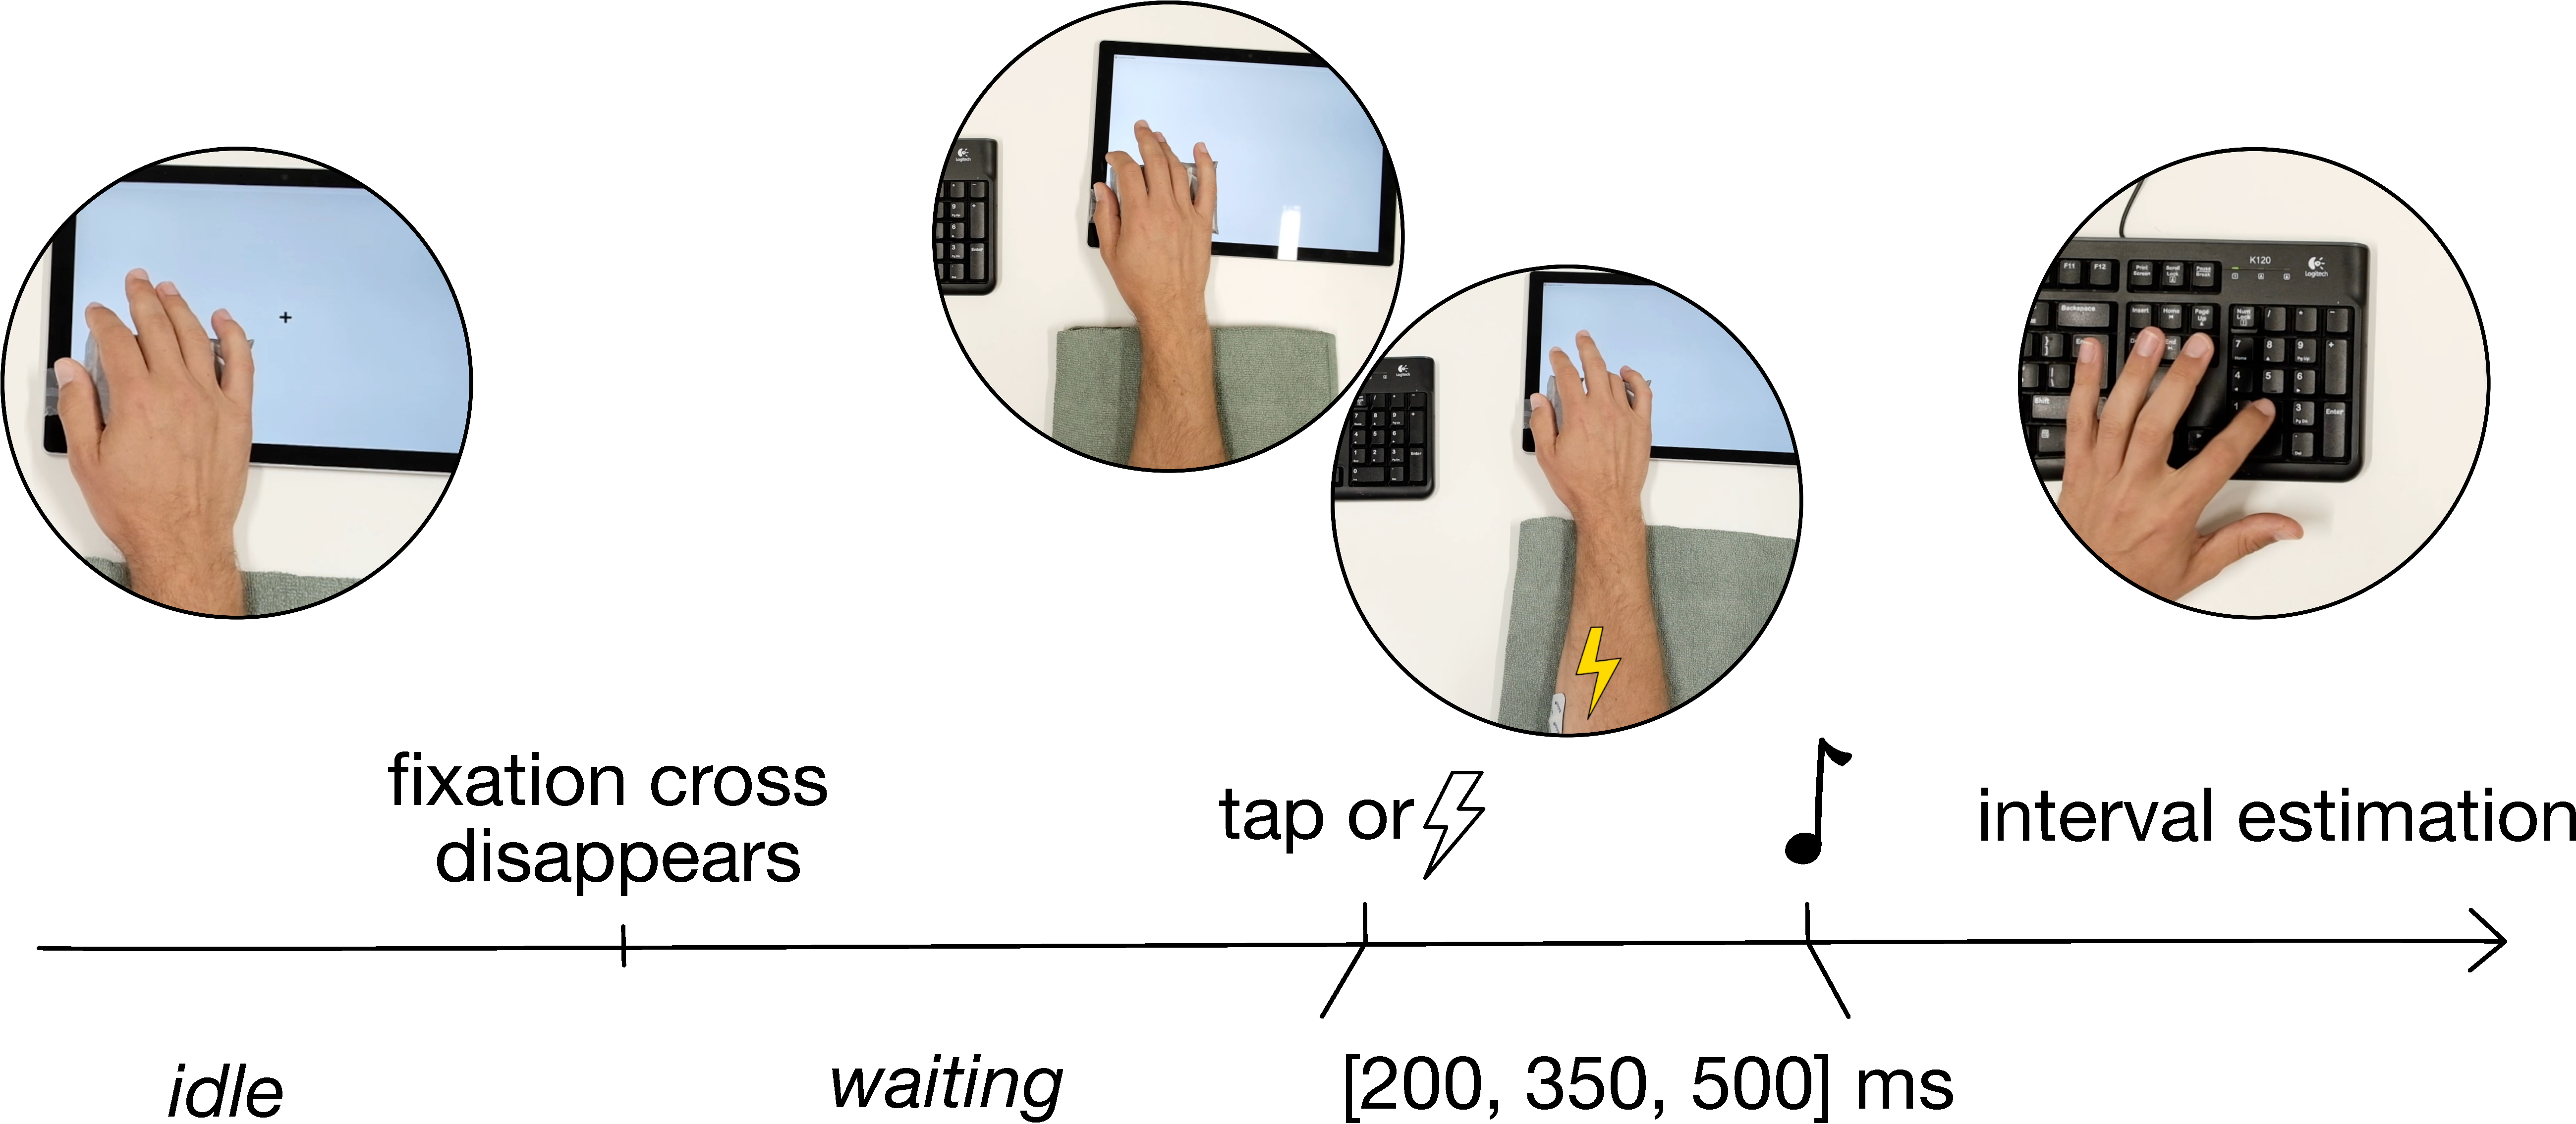
\includegraphics[width=\columnwidth]{figures/task_new.pdf}
    \caption{Interaction flow depicting one trial in our touchscreen tapping task.}
    \label{fig:progression}
\end{figure}

\indent\textbf{INTENTION.} The task went as follows: (1) a fixation cross appeared on a tablet screen and participants were instructed to rest and wait until it disappeared; (2) then, they were instructed to wait for a brief moment (2 to 3s), before (3) initiating their movement and tap the screen. In line with the literature on the origin of the RP generating process they were told ``to avoid pre-planning the movement, avoid any obvious rhythm over trials, and to press when they felt the spontaneous urge to move''~\cite{Schultze-Kraft2021-cu}. (4) After the screen was tapped, a tone was played at a pseudo-random delay of 200, 350, or 500ms. Participants were now asked to estimate the delay, typing in their answer on a number pad of an attached keyboard. After confirming their answer by hitting the return key, the next trial started.
During INTENTION, participants were equipped with Electromyogram (EMG) sensors instead of EMS electrodes. INTENTION data was used as training data for the BCI, see section~\ref{BCI} below, as well as to select stereotypical reaction times in the EXTERNAL condition. 

\indent\textbf{EXTERNAL.} The task structure was identical to INTENTION, however, participants were now instructed to hold and wait for the muscle stimulation to move their finger thereby eliciting the screen tap. The timing for the EMS trigger was taken by randomly choosing a time between the 5th and 95th percentile of their actual individual reaction time in the INTENTION condition. 

\indent\textbf{AUGMENTED.} The task and instruction were identical to INTENTION with one additional instruction: ``you will now work \textit{with} the system''. During AUGMENTED, the muscle stimulation hardware was controlled by the BCI. The classifier was set to active after the fixation cross disappeared and until a screen tap was registered. Hence, the muscle was not stimulated at other times during a trial, so as not to interfere with participants typing in their time estimation response.

The order of the conditions was not pseudo-randomized since training data obtained in INTENTION was required for both EXTERNAL and AUGMENTED. Furthermore, AUGMENTED was always the last condition, thereby allowing for a prolonged interview.

% \begin{figure*}
%     \centering
%     \includegraphics[width=\textwidth]{figures/task_design.png}
%     \caption{(a) description of the experimental conditions, (b) their hypothesized effects on sense of agency from the perspective of a comparator model, is inspired by~\citet{Dewey2019-dg} (c) depicts the flow of movement generation in the participant and the system between conditions.}
%     \label{fig:task_design}
% \end{figure*}

\subsection{Apparatus}
The experimental setup, depicted in Figure~\ref{fig:setup}, comprised: (1) a 1-channel EMG device, (2) a 64-channel EEG system, (3) a medically-compliant EMS device connected via two electrodes worn on the forearm, and (4) a tablet to run the experiment and collect behavioral responses. To assist readers in replicating our experiment, we provide the necessary technical details, the complete source code for the experiment, the collected data, and the analysis scripts\footnote{[anonymized]}.
% TODO add links after anonymization is lifted.

\indent\textbf{(1) EMG Recording.} EMG data was recorded from 1 bipolar channel using the BrainAmp ExG amplifier (BrainProducts GmbH, Gilching, Germany). The two electrodes were placed above the flexor digitorum profundus with a reference electrode located on the wrist bone. EMG data was collected in synchrony with the EEG data through BrainProducts BrainVision Recorder.

\indent\textbf{(2) EEG Recording.} EEG data was recorded from 64 actively amplified Ag/AgCl electrodes in an actiCap Snap cap using BrainAmp DC amplifiers from BrainProducts. Electrodes were placed according to the extended international 10–20 system \cite{Jasper1983-uw}. One electrode was placed under the right eye to provide additional information about eye movements (vEOG). After fitting the cap, all electrodes were filled with conductive gel to ensure proper conductivity, and electrode impedance was brought below 10$\Omega$. EEG (and EMG) data were recorded with a sampling rate of 250 Hz. 

We used LSL\footnote{https://github.com/sccn/labstreaminglayer} to make the data streams available in the network and synchronize the recordings of EEG/EMG data and an experiment marker stream that marked sections of the study procedure.

\begin{figure}[!h]
    \centering
    \includegraphics[width=\columnwidth]{figures/setup.png}
    \label{fig:setup}
    \caption{Experimental setup of measurement-- and input devices (image with consent from participant).}
\end{figure}

\indent\textbf{(3) Electrical Muscle Stimulation.} We actuated the ring finger via EMS, which was delivered with two electrodes attached to the participants' flexor digitorum profundus muscle. We utilized the flexor digitorum profundus since we found that we can robustly actuate it without inducing unintended motion of neighboring fingers. This finger actuation was achieved via a medically-compliant battery powered muscle stimulator (TENS/EMS Super Duo Plus, prorelax, Düren, Germany). The EMS system's output was controlled by flipping a solid state relay (silent) connected via an Arduino Uno (Arduino, Monza, Italy) to the experiment computer. The EMS was pre-calibrated by the participant to ensure a pain-free but effective stimulation and robust actuation leading to an `immediate' tap on the touchscreen after actuation. To ensure a comfortable experimental experience so that participants relaxed their arm musculature as much as possible, a custom built hand rest (support device) was placed on top of the touchscreen for participants, see figure~\ref{fig:setup}.
% [todo] What were the settings of the stimulation?

\indent\textbf{(4) Experiment Presentation and Collection of Behavioral Responses.} An Acer Group (Acer Inc, Taipeh, Taiwan) tablet was used to present the task to participants and record their behavioral responses. In addition to the tablet, we used an external keyboard to allow response input of users indicating their timing judgements.

% alternative headings:
% Brain-Computer Interface to Detect EEG Readiness Potentials }
% Classifiying EEG Signals of the Intent to Interact
\subsection{Brain-Computer Interface}\label{BCI}
The data obtained in INTENTION was used to train the BCI. We utilized the [anonymized] and the EEGLAB~\cite{Delorme2004-sn} toolbox inside the MATLAB (The MathWorks Inc. Natick, MA, USA) environment for preprocessing both EEG and EMG data. First, to generate behavioral labels at a high temporal resolution for the EEG-based classifier, we leveraged EMG data from the flexor digitorum profundus. EMG amplitudes were band-pass filtered from 20 to 100 Hz and subsequently squared. Next, in order to label the time of movement onset, the EMG data was averaged across trials for the second preceding the screen tap. From this averaged data, the first sample where the EMG amplitude exceeded the 95th percentile was selected as the time of movement onset.
% bemobil pipeline

% TODO Next, noisy data segments were determined. 
% A segment was rejected as an outlier using Matlab's \textit{isoutlier} function using default parameters. % from isoutlier documentation (mean segment amplitude exceeding 3 scaled median absolute deviation)

Two event classes were then defined as follows: \textit{pre-movement} from -1000 to 0 ms preceding the (EMG detected) movement onsets and \textit{idle}, a one-second data segment between trials where participants were looking at a fixation cross.

\subsubsection{Preprocessing EEG and Selecting discriminative channels}\label{eeg_methods}
The EEG data was band pass filtered from 0.1 to 15 Hz. In the first step to prepare the EEG data for classification, noisy data segments were rejected. To this end, the EEGLAB function `autorej' was used, keeping default parameters. A trial was excluded if \textit{either} data from the \textit{idle} or \textit{pre-movement} class was rejected.

Then, to decrease the dimensionality of the EEG data, a selection of discriminative channels was conducted following a selection approach outlined by~\citep{Schultze-Kraft2021-cu}. First, for both \textit{pre-movement} and \textit{idle} the mean signal in the last 100 ms of each segment was subtracted from the mean signal in the first 100 ms of the segment. The resulting value thus indicated how much the signal had changed in the course of the 1 s segments. In line with the literature, there should be a change over time in the \textit{pre-movement} segment but not in the \textit{idle} segment. Then, all channels were sorted (1) in descending order by the signal difference in the \textit{pre-movement} segments and (2) in ascending order by the signal difference in the \textit{idle} segments. With respect to the ability of the system to discriminate between movement intention and the absence of movement intention, an ideal channel should show a strong change in signal over the course of a \textit{pre-movement} segment but no difference during an \textit{idle} segment. The ranks of the two criteria were joined by summation and the resulting order was saved for later use in training and real-time application of the classifier. Lastly, channels C3, C4 and Cz were moved to the top of the order for every participant as these are most frequently reported in studies on the RP.

\subsubsection{Training of EEG classifier}
To classify EEG data a linear discriminant analysis (LDA) with shrinkage regularization (automatic shrinkage using the Ledoit-Wolf lemma~\cite{Ledoit2004-bi}) was trained for each participant individually. As single-trial features, the (linear) slope coefficient was obtained for both \textit{idle} and \textit{pre-movement} segments by fitting a linear regression. The classifier was then trained using the slope coefficient feature of the selection of the most discriminative channels as features, hence in the end, generating a feature vector in the dimension of channels that were kept for classification. We purposefully constrained the dimensionality of the feature vector to avoid over-fitting. 

Using scikit-learn~\cite{Pedregosa2012-sj}, an LDA with automatic shrinkage was cross-validated (using 5-folds) for a grid search from 6 to 20 channels with a step size of adding 2 channels. Following this grid search, the cross-validation with the highest accuracy determined the number of channels that were kept for training the model for real-time application. Ultimately, to determine the threshold at which, during real-time application, the classifier would trigger the EMS, we computed the Receiver-operator characteristic (ROC) and from this selected the threshold at 15 \% false positive rate.

\subsubsection{Real-time application and EMS control}
During real-time application, the EEG data was buffered for the last second for the selected channels. The data was band-pass filtered analogously to the training data from 0.1 to 15 Hz. Next, the slope was computed for the discriminative channels selected in the classifier cross-validation grid search. This procedure ran at an update rate of 10 Hz, hence every 100 ms a new prediction was obtained from the classifier. To smooth the prediction output with the goal of reducing false predictions due to unlikely peaks, the predicted probability for the \textit{pre-movement} class was smoothed by averaging the last two predictions with a weighting (.3 and .5). Then, at 10Hz update rate, this smoothed probability, as well as the predicted class for the current frame were gating the EMS switch: when the probability exceeded the threshold and the currently predicted class was \textit{pre-movement}, the switch was opened for 0.5s.

% To trigger the EMS, an Arduino was used to flip a switch whenever triggering the attached EMS. We constrained the times when the switch could be flipped to specific moments in the experiment where participants were getting ready to perform an action, thereby limiting the impact of distracting EMS pulses at resting phases during the experimental trials. %This guaranteed that participants experienced EMS only during movement preparation

\subsection{Measures of Agency Experience: Intentional Binding, Question \& Interview}
To assess if SoA was preserved, an intentional binding measure, a standardized question, and an interview following the AUGMENTED block were investigated. At the conclusion of each condition we prompted participants to rate their experienced agency on a 7-point Likert scale with the statement ``It felt like I was in control of the movements during the task.'', the item was copied from~\cite{Hornbaek}. Following AUGMENTED we interviewed users about their experience working with the system. After prompting users to recall their experience and summarize what their task had been we set the focus to the tapping movement and asked them to ignore the time estimation task for the following questions. We entered the open part of the interview by asking: ``What did the system do?'' followed up by ``What was the difference between the three conditions''. After some time, and depending on their answers, we reset the focus to the AUGMENTED condition and asked ``How often was the system active?'' followed by ``What do you think caused the actions of the system?''. This was then followed up by an `open' interview in which we frequently asked `how' and `why' questions to inquire about the user's experience.

% add back in after anonymization: All interviews were manually transcribed and then automatically translated using DeepL\footnote{https://www.deepl.com/translator}
We analyzed the interviews that always followed the AUGMENTED condition by loosely following~\citet{Mayring2015-pp}. All interviews were manually transcribed and [anonymized]. Prior to screening the texts, two experts clustered the responses into 3 clusters: First, ``Functionality'' referred to what participants attributed the source of the stimulation. Next, we clustered responses according to ``Guessed percentage'' of correct interaction, i.e., participants estimate of how well the system was aligned with their intention. For the cluster ``Correct Interaction'', we specifically queried participants to recall the moments where the stimulation felt in line with their intention to move, then we clustered their responses into positive and negative valence sentiments. 

\subsection{Statistical Analyses}
To confirm and demonstrate the discriminative power of the EEG features, we plotted the amplitude time course of electrode Cz between \textit{pre-move} and \textit{idle} epochs. Next, the slope coefficients were extracted and a paired t-test was conducted. Ultimately, to assess the classifier performance, we report the F1 score, i.e. the harmonic mean between of the precision and recall, and plot the ROC.

\subsubsection{Hypotheses Testing}
Prior to any statistical analyses of the intentional binding measure, outlier trials were rejected. We applied `extreme outlier removal' using Tukey's method~\cite{Tukey1949-sl}. Three time intervals were considered relevant to describe `regular' behavior across trials which would manifest by: (1) Tapping the screen in a reasonable interval after the fixation cross disappeared. An excessively short or long delay indicated that participants either tapped the screen prematurely by accident or they were checking in with the experimenter, respectively. (2) Providing a `reasonable' estimation in the intentional binding task. (3) The EMS stimulation leading to an \textit{immediate} screen tap. A long delay between the EMS trigger and the subsequent screen tap indicated that the stimulation was not strong enough in this trial to lead to muscle actuation resulting in a screen tap. Taken together, applying Tukey's methods to these criteria led to the exclusion of 102 trials across all participants (M = 34.00, SD = 16.46) and a final data set of 1698 trials.

In line with the literature on intentional binding, we hypothesized that the time intervals should be underestimated for the INTENTION and the AUGMENTED conditions. This should not be the case for the EXTERNAL condition where users had no intention to move. Hence, when binding occurs, the intervals should be underestimated, hinting at a higher SoA. To test this, we fit a linear mixed effects model with \textit{condition} (INTENTION, EXTERNAL, AUGMENTED) as a fixed effect. As a random effect, we considered the intercepts for participants. We obtained p-values of the coefficients by calculating likelihood-ratio tests~\cite{winterLinearModelsLinear2013}. All parameters were estimated by maximum likelihood estimation~\cite[see][]{Pinheiro2000}. Post-hoc, pairwise contrasts were computed using estimated marginal means with Tukey's methods for multiple comparisons corrections~\cite{Lenth2020-xk}.

Next, we hypothesized that subjective ratings of control over the tap movement are comparable between INTENTION and AUGMENTED and lower in the EXTERNAL condition. Again, we fit a linear mixed effects model with \textit{condition} as a fixed effect and participant ID as a random effect. Coefficients were assessed in the same way as for the intentional binding parameter above.

In short, we tested two main hypotheses with regard to experiencing agency in our three experimental conditions: (1) participants underestimate the tone delay when acting intentionally. Adding EMS in line with participants' intention to move does not affect this underestimation. (2) The subjective feeling of control is comparable between INTENTION and AUGMENTED conditions. EXTERNAL should decrease the feeling of control significantly. Additionally, we report the clustered interviews anecdotally.


%%% Resources
% An additional cluster ``takeaways'' was used to cluster other, miscellaneous,  interesting comments.

% "how did it feel like?". If user's made reference themselves to the EMS device we followed up by inquiring: "why do you think it (the EMS trigger) happened?", "What do you think triggered it?". The goal was to learn about the source attribution user's made about the EMS trigger. Since we leveraged the RP, we hypothesized that user's would attribute, at least in part, the EMS trigger to themselves, i.e. their movement intention. Next, we pressed deeper into learning about the cooperative nature between user and system. We asked "Do you believe you did it alone?" and when they made reference to a specific situation where the EMS was triggered we followed up with "What did it feel like, did you had the feeling the system controlled you or did you cooperate?" and "What would have to be there for it to feel like a cooperation?". We closed the interview with two additional exploratory questions: "Did the system influence your performance? If yes, how and why?" as well as asking them about any application scenarios they have in mind. 

% \indent\textbf{(1) Intentional Binding.}
% At the end of each trial participants were tasked to estimate the delay between the screen tap and a subsequent tone. The real delay was pseudo-randomized out of [200, 350 and 500] ms. With 75 trials per condition, each real delay occurred 25 times. 

% \indent\textbf{(2) Questionnaire.}

% \subsection{Brain-Computer Interface}
% The presented classification scheme required individual training data per participant, as transfer learning remains challenging with EEG~\cite{Wan2021-zz}. Therefore, we initially obtained training data on a variant of our task that did not include any muscle stimulation. In our task, participants were instructed, following an initial waiting period, to tap a touchscreen with their ring finger at their own volition, see figure ~\ref{fig:teaser}. 
% \subsubsection{Labelling movement classes using EMG}3

% Subsequently the data were labelled into two classes: an \textit{idle} class representing resting background activity and a \textit{pre-movement} class, representing the intent to (inter-)act.

% In summary, the experiment consisted of five phases: (1) a setup phase; (2) the BASELINE condition to obtain training data and labels; (3) the NO INTENTION condition: being passively moved by the EMS system; (4) the INTENTION EMS condition where the BCI was triggering the EMS system that in turn made participants tap the screen; and (5) an open interview to inquire about their experienced agency following the INTENTION EMS condition.

% \subsubsection{Experiment Design and Procedure}
% The first condition was used to obtain training data for the single-trial classification system. Here participants were wearing the EMG sensors instead of the EMS actuators and were instructed to tap the screen at their own volition (BASELINE, see instructions above). In the second condition, participants were instructed to hold and wait for the EMS system to move their finger thereby eliciting the screen tap (NO INTENTION). The timing for the EMS trigger was taken by randomly choosing a time between the 5th and 95th percentile of their actual reaction time in the BASELINE condition. In the third condition, the EMS trigger was controlled through the readiness potential classifier (INTENTION EMS). Participants were given the instruction: ``you will now work \textit{with} the system'' along the same instruction as in the BASELINE condition. The classifier was set to active after the fixation cross disappeared and until a screen tap was registered. Hence, the EMS was not triggered at other times during a trial, so as not to interfere with participants typing in their time estimation response.

% To not break the user's immersion by disturbing the flow of the interaction we decided against asking qualitative questions at the end of each and every trial.

% old:
% \subsubsection{Reproducing Results and Data Availability}
% Data, experimental protocol, analyses code including scripts for a reproduction of the presented results are hosted at open science foundation (OSF)\footnote{[anonymized]}. BIDS formatted data is hosted on openneuro~\cite{}.


% , and the interval between EMS stimulation and tap as fixed effects

% Hypothese:
% In line with the literature on intentional binding, we hypothesized this duration to remain stable in the case that agency was preserved during the test phase with EMS. A deviation of the tone duration from the training phase was hypothesized to reflect a disruption in experienced agency.

% operationalising temporal binding = underestimation (here or somewhere else) 

% \indent\textbf{(1) Hand Tracking.} We used an HTC Vive Tracker, attached to the participant's wrist, to track their right hand at 90Hz. Therefore, we ran a simple Unity3D scene and streamed the data via the labstreaminglatyer (LSL)\footnote{https://github.com/sccn/labstreaminglayer}

% At the end of each trial participants were tasked to compare the duration of their arm movement to a tone and indicate whether the tone was longer or shorter. We set the initial duration at 500 ms for each participant. When participants indicated the tone to be longer or shorter by pressing either the up or down key we added, or respectively subtracted, 100 ms from the tone duration. This new duration was then used for the next trial and so on. With 60 trials in the training phase, we hypothesized participants would oscillate 50-50 around a target duration after about 2/3 of the training trials. The final duration after all training trials was then used again as the start duration during the test phase. In line with the literature on intentional binding, we hypothesized this duration to remain stable in the case that agency was preserved during the test phase with EMS. A deviation of the tone duration from the training phase was hypothesized to reflect a disruption in experienced agency.


% (1) participants waited for a new letter to appear on screen; (2) then, they were instructed to wait for a brief moment (~2s), before (3) reaching out and pressing the key. In line with the literature on the origin of the RP generating process they were told "to avoid preplanning the movement, avoid any obvious rhythm, and to press when they felt the spontaneous urge to move". (4) Two \todo{how many, but do keep this constant in order for them to focus on the duration of their action} seconds after they pressed the key, they were presented with a tone and asked to judge whether their movement, from the start of their reach to the button press, lasted longer or shorter than the tone. (5) When they perceived the tone to be longer, they had to press the up key or vice versa the down key for perceiving that the tone was shorter than their movement. Following an inter-trial-interval the next trial started.

% For each trial, a key was randomly selected from one of two groups of letters: (1) 'a', 's', 'd' or (2) 'j', 'k', 'l'. The selected group was then changed with every trial. This was done to keep the task engaging while maintaining a comparable reaching movement between trials.

% ERP with significance mask for Cz? Assessing significance of classifier

% IB Task: ttest of final ib time between with and without EMS -> # subjects input values
% did they increase the IB task in more than 50% of the trials after EMS?

% questionnaires: ttest against zero to report direction

% interviews: anecdotal summary and sentiment analyses with two groups splitting questionnaires at 0

% correlation with EEG classifier accuracy?

% evaluation of EEG classifier: can report false negatives, how often was it missing to predict a movement onset? hand was moving without EMS being triggered occurred how often? Not possible to evlaute false positives as no ground truth available
\section{Results}
% We first report the performance of the classification system, as the system performance greatly impacts the subjective experience of the motor augmentation.

% \subsection{Behavior: Intentional Binding}
In the intentional binding task, i.e. the estimation of the time interval between tap and tone, participants generally underestimated the average real delay (350ms) in all three conditions (INTENTION M = -160.7 ms, SD = 88.1; INVOLUNTARY M = -135.3, SD = 110.3, AUGMENTED M = -162.4, SD = 113.8). The underestimation was not affected by the condition, see~\ref{fig:ib_task}.

% The condition influenced the estimation (${\chi^{2}_{(2)}} = 17.1, p < .001$), see figure~\ref{fig:results}a. Post-hoc tests revealed that the underestimation was less pronounced in INVOLUNTARY as compared to INTENTION ($beta = 22.6, p < 0.001$). This was also the case in INVOLUNTARY, with less pronounced underestimations of the time interval between tap and tone compared to AUGMENTED ($beta = 15.3, p = 0.018$). No difference was observed between INTENTION and AUGMENTED.

\begin{figure}[h]
    \centering
    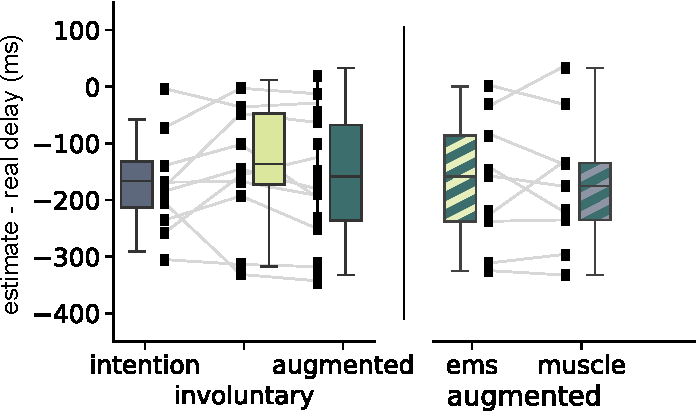
\includegraphics[width=\columnwidth]{figures/ib_task.pdf}
    \caption{Difference in time estimation from real delay in intentional binding task for the three experimental conditions (left). Negative values indicate a temporal compression, i.e., temporal binding. Right side: Trials in the AUGMENTED condition split in EMS-- and self-executed trials.}
    \label{fig:ib_task}
\end{figure}

\subsection{Subjective Ratings \& Reports}
The subjective rating of control differed between conditions (${\chi^{2}_{(2)}} = 43.7, p < .001$), see figure~\ref{fig:loc}b. Post-hoc tests revealed that participants rated their level of control higher in INTENTION compared to INVOLUNTARY ($beta = 4.8, p < .0001$), and higher in INTENTION compared to AUGMENTED ($beta = 3.1, p < .0001$). Further, higher control was observed in AUGMENTED compared to INVOLUNTARY ($beta = -2.9, p = .006$).

% \begin{figure}[h]
%     \centering
%     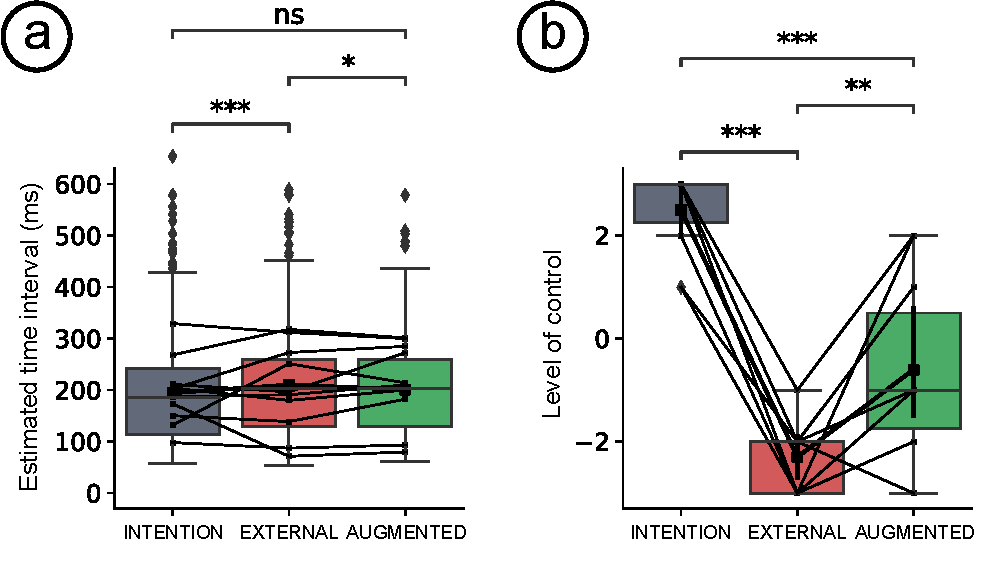
\includegraphics[width=\columnwidth]{figures/subjective_results.pdf}
%     \caption{(a) Temporal binding effect over conditions. With an average presented time interval of 350ms, lower values in the estimated time interval indicate an underestimation, i.e., temporal binding. (b) Subjective ratings of control across conditions. Significance labels obtained from post-hoc tests on estimated marginal means.}
%     \label{fig:results}
% \end{figure}

\begin{figure}[h]
    \centering
    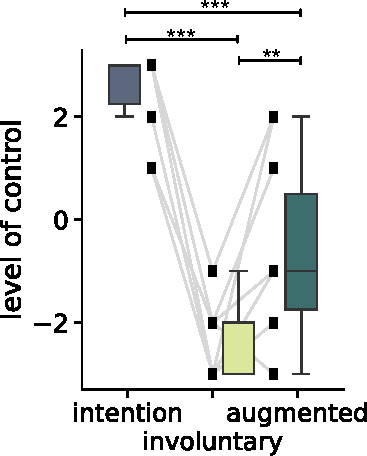
\includegraphics[width=.5\columnwidth]{figures/level_of_control.pdf}
    \caption{Subjective ratings of control across conditions. Significance labels obtained from post-hoc tests on estimated marginal means.}
    \label{fig:loc}
\end{figure}

\paragraph{Functionality.} Eight out of the ten participants made a reference to the source of the EMS in the AUGMENTED condition. In that subgroup, most participants wondered how the system worked, one remarked, ``I can't explain how it works technically.''. Another one mentioned that ``maybe the time estimation task had something to do with it.''. They found the stimulation to be sporadic, even during their own actions, leading to a belief that it was coincidental. As one participant put it, ``I have no idea what controlled the stimulation, I think it was coincidence when stimulation occurred.''. Furthermore, participants reported that they found the timing of the stimulation to be unpredictable, with one participant noting, ``Stimulation was random in time.''. 

Some perceived the stimulation as externally triggered, yet partially responsive to their choices, resulting in a sentiment captured by, ``I think that the stimulation in the third block was partly random, but partly as if it was following my decision/choice.''. One participant noted that they felt that ``somehow the information is in my arm''. Another one briefly considered the involvement of their brain waves in controlling the stimulation, but expressed doubts about this possibility, stating, ``But I don't think that is the case.''.

\paragraph{Guessed Percentage.} 
Some participants reported that the stimulation ``sometimes overlapped with the movement, but not often,'' or, it ``came only rarely.'' Another one noted, ``In a few cases, the stimulation came when I had already started the movement.'' For several participants, this overlap between their actions and the system's response occurred infrequently, with another user noting, ``Once, in the millisecond range between my planned movement and its execution.'' However, for some participants, there were moments of near-perfect synchronization, as described by one participant, ``In 3 cases it happened that my intention to press and the impulse of the device happened simultaneously.'' or ``in 3--4 cases it happened simultaneously that i wanted to tap and the stimulation happened''. Another one noted, ``Sometimes it really happened that they overlapped. So that I just started to move, and then the device activated,'' that user estimated an overlap of ``40 \%'' while two other users said [we worked together in] ``15 \% of trials.'' These accounts collectively highlight the varied and occasionally synchronous nature of the system's timing in relation to the users' intentions.

\paragraph{Correct Interaction.} 
In terms of valence sentiments for the cases where the stimulation aligned with participants' intentions, some participants indicated that the experience was positive, for example, participants described the experience as ``rather funny'', ``weird but funny'', ``pleasant'' or ``helped me with the execution'' and ``it was more of a collective movement.'' One participant remarked ``then it was ok to experience the stimulation, but also not more than ok'' while another one noted ``It had a bit of thinking ahead to it''. Some noted that they experienced an increase in their physical strength, remarking, ``supported my strength'', ``made me type more firmly'' and ``my typing performance was increased.'' On the other hand, some participants had negative sentiments during these moments of aligned stimulation, remarking, ``felt like I was still in competition with the system'', ``it did not feel like an acting together'' and ``on a psychological level it was a loss of control.'' Another one noted, that they ``felt determined-by-others and then tried to resist the impulse. I felt excluded from the decision to tap''.

\subsection{Classifier Performance}
Visual inspection of the amplitudes at electrode Cz revealed an increase in the difference between \textit{pre-movement} and \textit{idle} data segments towards the onset of the finger movement, see figure~\ref{fig:EEG_results}a. The slope feature for the exemplary channel Cz discriminates well between the two classes (${t_{(10)}} = 4.4, p < .001$), see figure ~\ref{fig:EEG_results}b bottom. The scalp maps in figure~\ref{fig:EEG_results}b top show the (color-coded) mean slope for each channel and each class. Central channels on the contralateral side to the moving finger on the right hand show a negative slope for the pre-movement class and a neutral slope for the idle class. Furthermore, differences in slope were also observed at frontal electrodes over the left hemisphere as well as parietal electrodes, were a positive slope manifested only for the idle class. 

\begin{figure*}[t]
    \centering
    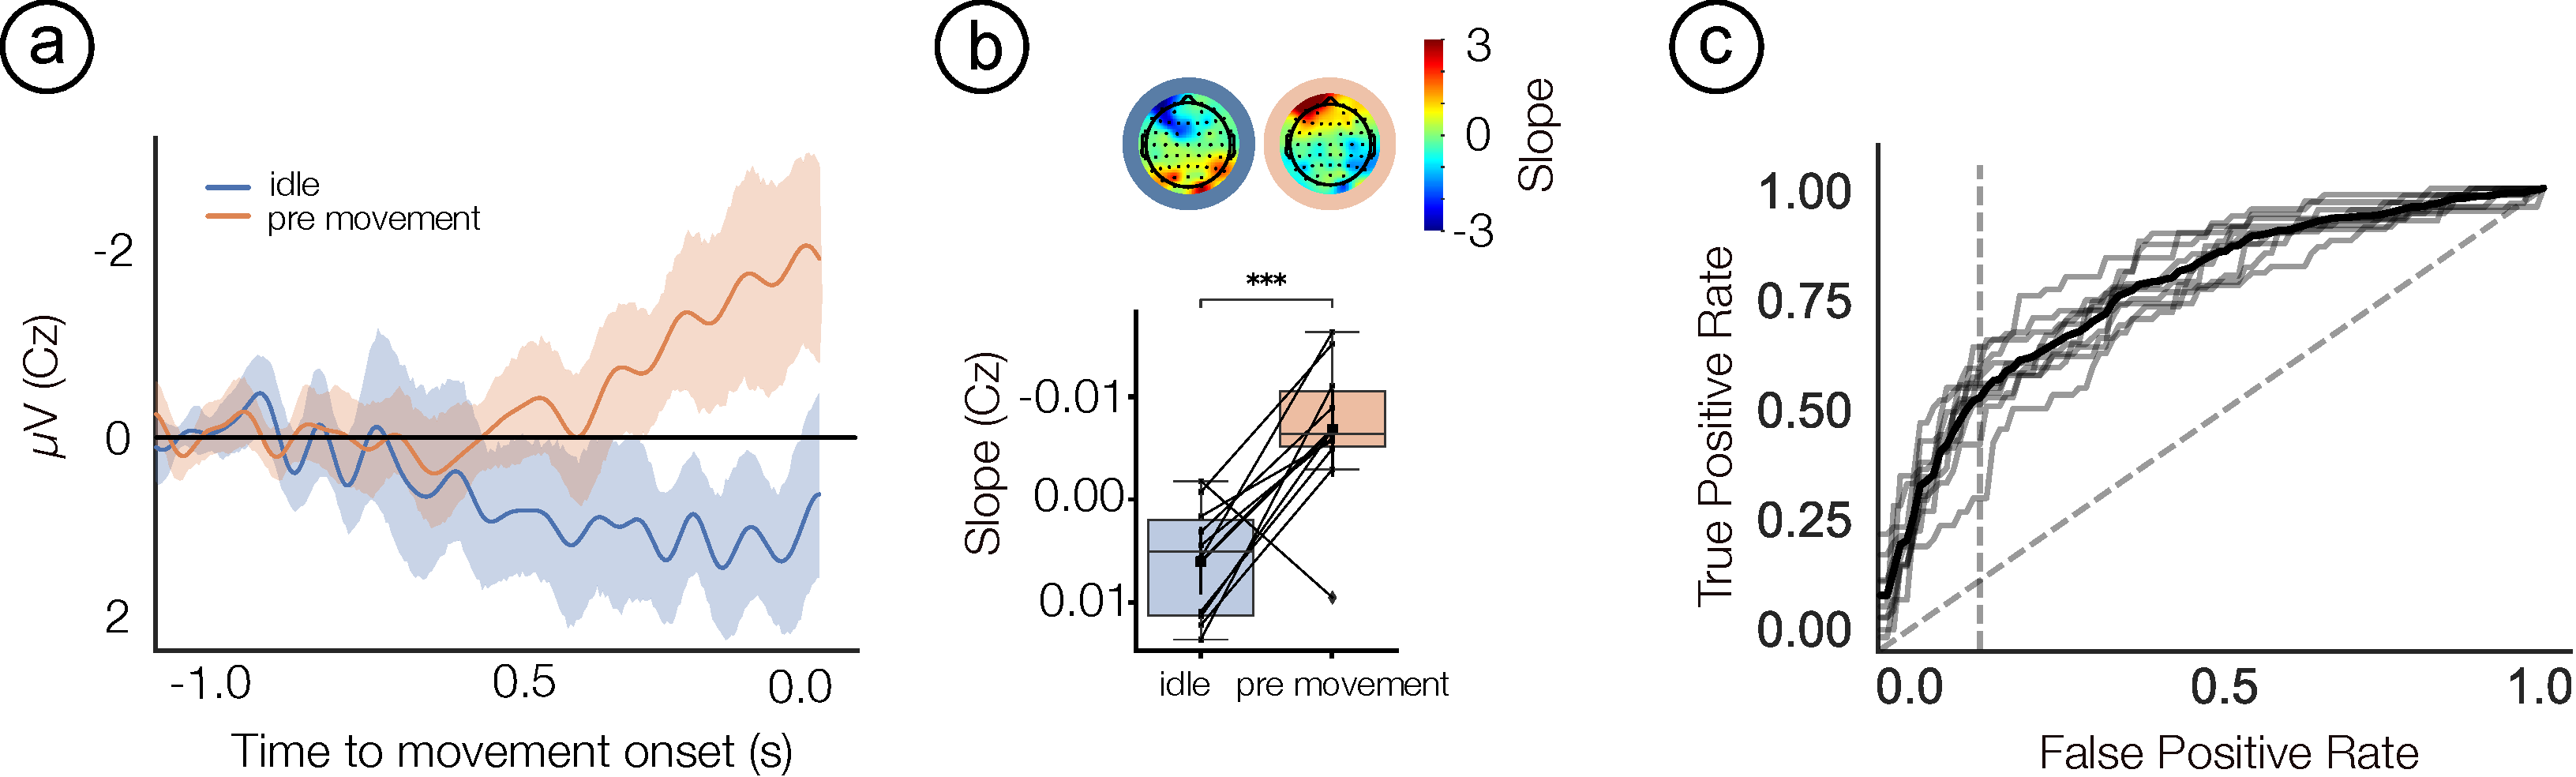
\includegraphics[width=\textwidth]{figures/eeg_results_new.pdf}
    \caption{(a) Grand average event-related potential (ERP) at electrode Cz of pre-movement EEG data epochs preceding the last second before a movement, idle epochs of the same trial are plotted alongside but originate from a different time window, see section~\ref{eeg_methods}; (b) Bottom: Slope features for both idle and pre-movement classes at electrode Cz. Top: Scalp maps of slope values for both classes and all channels. (c): Mean and per participant ROC curves. Dotted line at 15 \% false positive rate indicate the selected threshold for the real-time application.}
    \label{fig:EEG_results}
\end{figure*}

The grid-search over channels resulted in the BCI leveraging on average 11.2 (SD = 3.6) channels. Besides channels C3, C4, and Cz, that were always included, other common channels (retained for at least 3 participants) included FT9 and AF3. The classifier cross-validation resulted in a mean F1 score of .71 (SD = .03), see figure~\ref{fig:EEG_results}c. We set the detection threshold to 15 \% false positive rate and at that rate, observed a mean threshold of 57 \% (SD = .04). Hence, on average, the classifier switched on the EMS when it predicted class \textit{pre-movement} with 57 \% probability.

\subsubsection{Post-hoc analyses of classifier performance}

In line with the readiness potential a negative going deflection over the last second preceding the movement onset was present in both INTENTION and AUGMENTED, but not in INVOLUNTARY, see figure~\ref{fig:erp}a. Furthermore, ERPs differed between the three conditions in the time window from 210 ms -- 250 ms following movement onset ($\chi^{2}_{(2} = 10.6, p = .03$ at 220 ms). INVOLUNTARY exhibited a strong negativity peak (strongest among the three conditions), peaking at around -10 $\mu$V at 210 ms after movement onset. A weaker peak was observed for AUGMENTED (-6 $\mu$V at 210 ms) and even more so for INTENTION (-2 $\mu$V at 150 ms).

\begin{figure}[h]
    \centering
    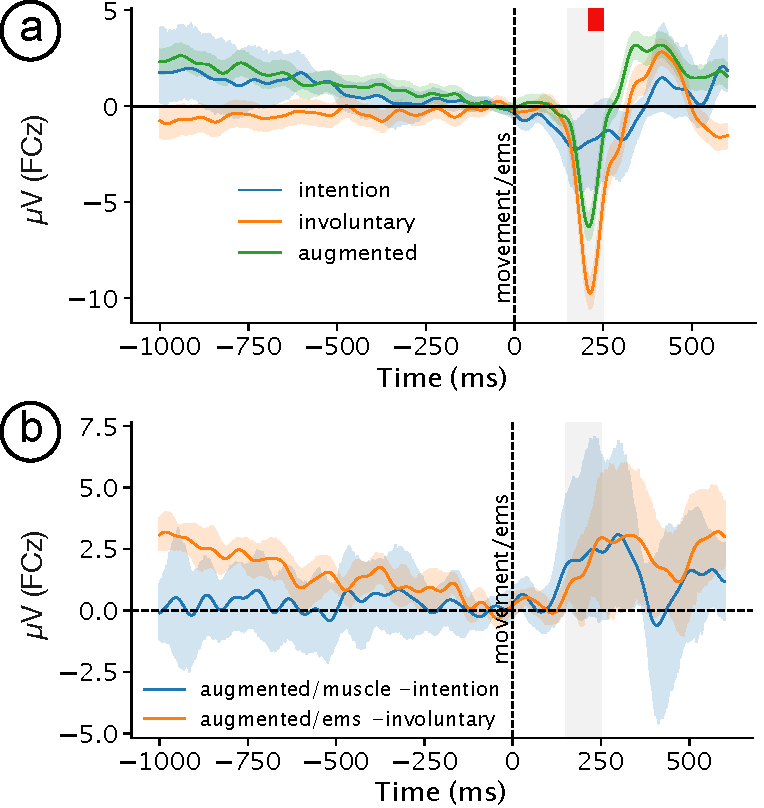
\includegraphics[width=\columnwidth]{figures/PE_erp.pdf}
    \caption{ERPs at electrode FCz from -1000 before, to 600 ms after the tapping movement onset. Top (a): INTENTION, INVOLUNTARY and AUGMENTED trials. Red bar on top indicate main effect at $p<.05$. Bottom (b): Difference ERPs at FCz of the `muscle-controlled' trials in AUGMENTED minus INTENTION as well as EMS trials in AUGMENTED minus INVOLUNTARY.}
    \label{fig:erp}
\end{figure}

When correcting for the influence of the EMS by subtracting INVOLUNTARY from EMS trials in AUGMENTED an INTENTION from `muscle-controlled' trials in AUGMENTED we observed no differences. Visually, it appears that trials in both INVOLUNTARY and INTENTION condition exhibit a stronger negativity in the post movement time window of interest than respective EMS and `muscle-controlled' trials in AUGMENTED, see the positive deflections peaking at 300 ms post movement onset in figure~\ref{fig:erp}b.



%%% Resources and Ideas
% and the agency condition by xx (CI: ). Subsequent non-parametric comparisons revealed the significance of differences only between  
% xx (p = ).
% x\



%\missingfigure{A: Boxplot of questionnaire scores of three Blocks (block 2 grey, because not intention given) - play around with visualization of words that were used to explain control rating. B. Boxplots intentional binding (maybe integrate A and B) C. more subjective evaluation of interview / maybe world cloud / maybe sentiment analysis) } 



% Did they get faster? Calculate time between hand motion onset and button press. If yes, evidence that there was acceptance for the help/augmentation the system provided

\section{Discussion}
With this paper, we contributed a new way to design \textcolor{green}{the experience of action augmentation}\textcolor{red}{augmented experiences} with the potential to maintain a user's SoA: a BCI to control EMS at moments of users' intention to interact. By leveraging an average of 11.5 EEG channels and using a simple, fast-to-compute feature, the BCI achieved a mean F1 score of .7. We demonstrated in eight participants that one effect of SoA, intentional binding, is maintained when using our system. However, the subjectively rated level of control was lower when using the system as compared to voluntary interaction without EMS. This was differentiated by participants' qualitative reports: when the stimulation aligned with participants' intentions, positive sentiments outweighed negative ones. When it did not, participants reported a negatively perceived loss of control.

% Sandwich: 
% Good -> [short] cool system, first of its kind setting out to augment user's action preceeding their movement in time
Our system was built using off-the-shelf, affordable, equipment to physically augment users' actions. Taken together, all technical devices to control the users' movements, i.e., the EMS stimulation device, Arduino, and switchboard, cost less than 100 Euros. While we used a 64-channel research-grade EEG system, the channel selection procedure resulted in the system ultimately using a low-density coverage of about 12 channels on average for classification. Today, many low-density EEG devices are available on consumer markets at affordable price points, see~\citet{Niso2023-ce} for a recent summary of available wireless systems. 

Still, the system achieved what is considered to be a `good' F1 score of .7, and hence sometimes detected users' intention to interact. In our user study, this system performance affected users' \textcolor{green}{tendency for temporal binding}\textcolor{red}{performance in the time estimation task} when comparing the three experimental conditions. We conclude that, taking users' sentiments and ratings of control into account, this indicates a general modulation of agency for our intention-based augmentation. We believe this to be a very promising finding because our prototype with low technological requirements still produces behavioral results indicating that intention can be detected and planned movements be augmented.

\textcolor{green}{Our system ran at a 10 Hz update rate. This was chosen in order to avoid buffer overflow due to the fact that the end-to-end computing latency from measuring the physiological signal to outputting the predicted class and probability took about 40 ms. The RP is reported to occur several hundred milliseconds prior to the physical movement~\cite{Schurger2021-vp}. Therefore, our augmentation should have resulted in a motion preemption, considering subtracting the computing latency and a delay that the EMS stimulation takes to affect the muscle from the RP-based intention detection. However, it is difficult to assess whether participants movements were in fact pre-empted as no label exists for the `true' intention onset to compare the classifier to. That participants were able to act on their own volition, and hence no labelling of their movement intention could be derived, is the key distinction to related works using controlled stimulus-response paradigms.}

\textcolor{green}{However, we learned from these paradigms that increasing participants reaction times by about 80 ms is optimal with regards to maintaining SoA~\cite{Kasahara2019-sk}. On one hand our system is capable of delivering pre-emption within this `SoA-optimal' time range. On the other hand however, the performance of the sub-optimal performance of the classifier means a lot of variation due to false positive detections. While in some cases, as we observed in the users' comments, the stimulation may have pre-empted a user's motion, false positive stimulation may have had a significant impact on the overall impression of the system, see section~\ref{improving_classifier} below.}

In line with the literature, we found that participants estimated the delay between tap and tone to be lower in both conditions where they were instructed to act on their own volition as compared to the passive condition~\cite{Moore2012-dk}. We point out that recent literature has questioned the validity of the intentional binding phenomenon as a correlate of agency, stating that the effect may ``merely represent a strong case of multisensory causal binding.''~\cite{Suzuki2019-pi, Gutzeit2023-ei, Hoerl2020-my}. However, in our study, we observed the effect of compressing the action-outcome delay to be maintained even when using the system. Hence, the effect was maintained for both conditions of voluntary action.

% Bad -> (1) situate the findings of the IB, (2) bad classification metrics not good enough to feel in control
\subsection{Limitations}
Two main procedural issues arose concerning the time estimation task: First, contrasting AUGMENTED with INTENTION, we noted that when EMS moved participants' fingers, they sometimes reported that their finger was pressing on the touchscreen for a longer duration as compared to their `normal' touchscreen tap. This may have introduced additional variance in the time estimation task since the exact moment of the tap that causes the tone is more obscure. Second, following pilot recordings, we chose to obtain participants' time estimates by asking them to type in their estimates on the keyboard. However, we observed that many participants, while perceiving a continuous distribution of the delays, did not answer at a continuous ms resolution but rather at steps of 50 or 100 ms, skewing the distribution of their answers. While many different versions of the intentional binding paradigm exist~\cite{Moore2012-dk}, we would choose a continuous slider for future experiments with different initial positions over trials to reduce the bias in participants' estimates.

\subsubsection{Improving the Prediction of the Intent to (Inter-) act}\label{improving_classifier}
While an F1 score of .7 may be considered `good' for many classification scenarios, when aiming to elicit a feeling of control this level of performance may likely not be good enough, see~\citet{Papenmeier2022-oi} for a review. Balancing false positive rate (FPR) and true positive rate (TPR) appropriately may prove crucial to elicit an experience of agency.

For the current study, we must note the following limitations arising from the (potentially) insufficient performance of the classification system. To provide a full picture we first describe the impact from a signal detection point of view: False negative classifications meant that the system did not trigger an EMS pulse in line with participants intent to tap on the screen. On the other hand, false positive classification meant that an EMS pulse was sent in the absence of a true intention by the participant. Both cases, individually and jointly, had the potential to significantly impact the user experience and erode trust in the system. In the interviews, participants reported only a relatively low number of correctly detected intentions. This may have ultimately led to a misalignment between users' perceptions and the observed, measurable, system behavior. 

As a consequence, the insights gained into the system's potential to preserve a sense of agency are limited. The quantitative metrics employed in our study, specifically those measuring the sense of control (including temporal binding and item assessment), may not have captured the nuanced temporal alignment experiences associated with EMS augmentation and user movement intentions but rather a more holistic assessment of the entire experimental block, which included trials with missed stimulation, too early stimulation, and some trials where the stimulation was in alignment with the participants' intent.

% Good -> This can be improved by using Gaze Dynamics, EMG and other things
% If it would work, how can it be used? Implications -> playful experiences, adaptive interfaces
Hence, a \textit{key} objective remains in improving the overall performance of the classification system. This can be accomplished by fusing several complementary models. For virtual reality (VR) platforms,~\citet{David-John2021-vg} have recently shown that gaze dynamics, especially gaze velocity, carry information with respect to the intent to interact. Furthermore,~\citet{Nguyen2023-me} presented further evidence that physiological signals originating from muscle activity (EMG) provide a very reliable label of movement onset~\cite{Nguyen2023-me}. Arguably, an augmentation system based on several models tuned to specific physiological features will reach sufficient classification performance in the very near future.

% Conclusion
\section{Conclusions}
In this paper, we demonstrated a system to maintain users' SoA during augmented experiences using brain signals reflecting the intent to (inter-) act. In our user study, we found that intentional binding effects were stronger when participants worked with the system to tap on a screen compared to when they were passively moved. Furthermore, the level of control working with the system was higher than when being passively moved, as indicated by subjective responses.

We believe this to be an important next step towards augmented users with full integration of the technology~\cite{Mueller2020-dl}. Ultimately, our closed-loop system enables novel predictive interfaces that leverage the users' body directly yet still feel \textit{natural} as they align with the users' intention: For example, altering the affordance structure of the interaction in real-time~\cite{Gehrke2022-kz, Lopes2015-ze, Nataraj2020-wm}.

With AI technologies becoming more and more ubiquitous in our everyday lives, questions about how agency is shared between us humans and AI technologies arise regularly. With the likely future that these systems move directly onto our bodies, alignment with users' intentions will be the \textit{key} component driving their adoption.





\begin{comment}
% Kasahara work, Tajima, neuromodulation? reference my affordance position paper -> copy text from there!! or during painting -> scott/gehrke -> reuse image?, affordance ++ as well, 
- relevance of research for prostheses ( see https://link.springer.com/chapter/10.1007/978-3-030-38740-2_8)
% At this point in time, the movement plan is already in place and so <[rework] there is slack in the perceptual system that can be exploited so user's action can be altered with them noticing>. 
- EMS augmented interaction might make sense for bigger movements (e,g. back muscle to support lifting) -> might have less effect (negative) effect on the feeling of control, since it is a less specific movement
- However, brain signal might not be the best indicator in such cases (simply motion tracking indicating the start of the movement)

% playful experiences: EMS 

\missingfigure[]{Hand weg zieh spiel foto, beispielhafte playful experience in der es interessant ist mit dem agency konzept herumzuspielen und es spielerisch zu entdecken?}

- a bit on HCINT?
% What do I want to say here? Just in general describe the level of integrations that exist and then say where we would place our prototype? Or is this more interesting for a later discussion part? Maybe yes, just move this to a later stage, it does not really add here and better fits in the discussion, also then to discuss the results and what it means to be integrated in a certain way

%- not only physical integration but also other adpative interfaces, or control of mobile phone (see Cornelio2022 review); % say here somewhere what action augmentation is and how it differs from body and environment/outcome augmentation

% briefly summarize the papers on discriminating action augementation and other such things, reference cornelio 2022 paper
% Previous research on augmented technology and ideas to maintain sense of of agency
% The experience of being integrated with a technology, or of being one ``human-technology assemblage'' <REF where is this from, Danry2022 used it> 

% Action augmentation technology using motor actuation aims to augment the user’s actions diminishing the SoA (see Cornelio 2022). 
% - add research
% Here I want to say where our system lies within the design space of augmentation devices and <cornelio2022> gives a good nomenclature for this. Then transition over to how agency is important to consider when localizing our prototpye and then in the next paragraph talk about what agency from a neuroscientific perspective
\end{comment}
% \section{Conclusions, Limitations and Opportunities}


% \section{Introduction}

% % First Paragraph
% % CORE MESSAGE OF THIS PARAGRAPH:
% \todo{P1.1. What is the large scope of the problem?}
% \todo{P1.2. What is the specific problem?}

% % Second Paragraph
% % CORE MESSAGE OF THIS PARAGRAPH:
% \todo{P2. The second paragraph should be about what have others been doing}
% \todo{P2.3. Why is the problem important? Why was this work carried out?}

% % Third Paragraph
% % CORE MESSAGE OF THIS PARAGRAPH:
% \todo{P3.4. What have you done?}
% \todo{P3.5. What is new about your work?}

% % Fourth paragraph
% % CORE MESSAGE OF THIS PARAGRAPH:
% \todo{P4.6. What did you find out? What are the concrete results?}
% \todo{P4.7. What are the implications? What does this mean for the bigger picture?}

% \section{Related Work}


% \section{Study Design}


% \section{Results}

% \section{Discussion}


% \section{Conclusion}


%%
%% The acknowledgments section is defined using the "acks" environment
%% (and NOT an unnumbered section). This ensures the proper
%% identification of the section in the article metadata, and the
%% consistent spelling of the heading.
\begin{acks}

% no section, just write down the acknowledgements as text\

ChatGPT (OpenAI, San Francisco, USA) was used to copy-edit author-generated content.
\end{acks}

%%
%% The next two lines define the bibliography style to be used, and
%% the bibliography file.
\bibliographystyle{ACM-Reference-Format}
\bibliography{input/paperpile}


%%
%% If your work has an appendix, this is the place to put it.
%\appendix
%\section{Research Methods}


\end{document}
\endinput
%%
%% End of file `sample-manuscript.tex'.
